\chapter{Electrostatics}

\section{The Electric Field}

\subsection{Introduction}

The fundamental problem in electrodynamics is how \vocab{source charges} $q_1,q_2,\dots$ (whose positions are \textit{given} as functions of time) affect a \vocab{test charge} $Q$ (whose trajectory is to be \textit{calculated}).

The \vocab{law of superposition} helps: the net force $\vec{F}$ on $Q$ is just the vector sum of the forces $\vec{F}_i$ from $q_i$ on $Q$:
\[\vec{F}=\sum_i \vec{F}_i.\]

Sadly, each individual force $\vec{F}_i$ is not easy to calculate, either. Indeed, it depends not only on the separation distance $\scr$, but also \textit{both} their velocities and on the \textit{acceleration} of $q$. Further, electromagnetic ``news" only propagates at the speed of light, so we need to consider \textit{not} what each $q_i$ is doing now, but what it was doing at some slightly earlier time.

So we need to simplify the problem. In \vocab{electrostatics}---as the name suggests---we take all the source charges $q_i$ to be static, or stationary (the test charge $Q$ can still move).

\subsection{Coulomb's Law}

Recall:

\begin{theorem}[Coulomb's Law]
The force of a stationary charge $q$ on a test charge $Q$ that is $\scr$ away is given by
\[\vec{F}=\frac{1}{4\pi\varepsilon_0}\frac{qQ}{\scr^2}{\hat{\scr}}.\]
This is confirmed by experiments. 
\end{theorem}

\begin{definition}
The constant here is
\[\varepsilon_0=8.85\times 10^{-12}\frac{\text{C}^2}{\text{N}\cdot\text{m}^2},\]
called the \vocab{permittivity of free space}.
\end{definition}

Notice that the force $\vec{F}$ is repulsive if $q$ and $Q$ have the same sign, and attractive if they have different signs. Indeed, $\vec{\scr}$ points from $q$ to $Q$.

\subsection{The Electric Field}

Now suppose we have $n$ source charges $q_1,q_2,\dots,q_n$, with respective vectors $\vec{\scr_1},\vec{\scr_2},\dots,\vec{\scr_n}$ to a test charge $Q$. Then, by the superposition principle, we have that
\[\vec{F}=\sum_{i=1}^n\vec{F}_i=\frac{Q}{4\pi\varepsilon_0}\sum_{i=1}^n\frac{q}{\scr_i^2}\hat{\scr_i}.\]
Notice how this quantity is proportional to $Q$, so we can define another vector field that depends \textit{only} on the source charges:
\begin{definition}
We define the \vocab{electric field} generated by source charges $q_1,\dots,q_n$ at a point $\vec{r}$ as
\[\vec{E}(\vec{r}):=\frac{1}{4\pi\varepsilon_0}\sum_{i=1}^n\frac{q_i}{\scr_i^2}\hat{\scr_i}.\]
\end{definition}
Then, the force of a test charge $Q$ placed at $\vec{r}$ is $\vec{F}=Q\vec{E}$, by the definition of $\vec{E}$. Further, since $\vec{E}$ is independent of any test charges $Q$, we can imagine it as an actual ``real" physical field that permeates space, and when test charges $Q$ are placed in the field they get pushed along (or against) the electric field.

\subsection{Continuous Charge Distribution}\label{contchardist}

We have only covered the case where the source is a collection of discrete point charges: to cover the continuous case, we need to turn our sum into an integral:
\[\vec{E}(\vec{r})=\frac{1}{4\pi\varepsilon_0}\int \frac{dq}{\scr^2}\hat{\scr}.\]
\begin{itemize}
    \item If the charge is spread over a line, with linear charge density $\lambda$, then $dq=\lambda d\ell'$, so
    \[\vec{E}(\vec{r})=\frac{1}{4\pi\varepsilon_0}
    \int\frac{\lambda(\vec{r'})}{\scr^2}\hat{\scr}d\ell'.\]
    \item If the charge is spread over a plane, with surface charge density $\sigma$, then $dq=\sigma da'$, so
    \[\vec{E}(\vec{r})=\frac{1}{4\pi\varepsilon_0}\int\frac{\sigma(\vec{r'})}{\scr^2}\hat{\scr}da'.\]
    \item If the charge is spread over a volume, with volume charge density $\rho$, then $dq=\rho d\tau'$, so
    \[\boxed{\vec{E}(\vec{r})=\frac{1}{4\pi\varepsilon_0}\int\frac{\rho(\vec{r'})}{\scr^2}\hat{\scr}d\tau'}.\]
\end{itemize}

Often, the final boxed equation is referred to as ``Coulomb's Law": it is not far from our original formulation, and volume charge distributions are common.

\section{Divergence and Curl of Electrostatic Fields}

\subsection{Field Lines, Flux, and Gauss' Law}

In principle, we are done with electrostatics: just compute the boxed integral above to find the electric field generated by the source charges; we know that a test charge $Q$ will simply receive a force $\vec{F}=Q\vec{E}$ at a point with electric field $\vec{E}$.

However, that integral is often intractable, so much of electrostatics is actually concerned with \textbf{assembling a bag of tools and tricks} to avoid them.

One tool to get a feel for electric fields is through \vocab{field lines}. We consider the case of a single point charge $q$ at the origin; shown below are (a) some vectors in the electric field and (b) electric field lines.

\begin{center}
    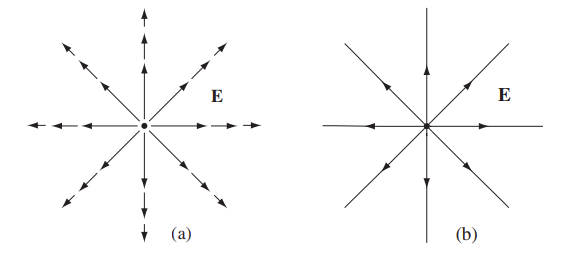
\includegraphics[width=12cm]{Electrodynamics/images/fig2.12.PNG}
\end{center}

It may seem like we lost some information: the strength of the field. However, we actually haven't! It turns out the magnitude of the field is indicated by the \textbf{density} of the field lines. However, the picture is actually a bit deceptive when drawn in two dimensions: it seems like the field drops with $1/r$; however, in three dimensions, we do get the correct $1/r^2$.

Note that charges must have a number of field lines emanating/terminating at it proportional to the magnitude of the charge. Further, electric field lines cannot terminate at any points other than charges (else $\nabla\cdot\vec{E}=0$, something we'll prove later, would be violated): they must start/end at charges or at infinity. Further, field lines cannot cross (otherwise the electric field at that point would have two directions!). Depicted below are the field lines for an electric dipole.

\begin{center}
    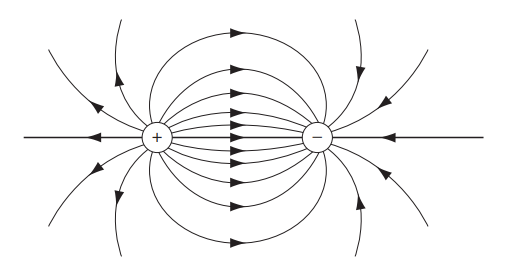
\includegraphics[width=10cm]{Electrodynamics/images/fig2.13.PNG}
\end{center}

Further, using this model, there's a simple interpretation for the \textit{flux} of $\vec{E}$ through a surface $\mathcal{S}$:
\[\Phi_E=\iint_{\mathcal{S}}\vec{E}\cdot d\vec{a}\]
is simply the (signed) number of electric field lines passing through $\mathcal{S}$.

This suggests that the flux through a \textit{closed} surface should measure the total charge inside the surface; in particular, charges outside should have no affect on the flux since any field lines that enter simply exit again.

This is the essence of \vocab{Gauss's law}.

\begin{theorem}[Gauss's Law]
    For any closed surface $\mathcal{S}$, we have
    \[\oiint_{\mathcal{S}}\vec{E}\cdot d\vec{a}=\frac{Q_{\text{enc}}}{\varepsilon_0},\]
    where $Q_{\text{enc}}$ is the total charge enclosed within $\mathcal{S}$.
\end{theorem}

Note that since Newton's law of gravitation also obeys $1/r^2$ fall-off, it will also obey an analogous Gauss's law.

To turn this into differential form, we can rewrite the left hand side using the divergence theorem:
\[\oiint_{\mathcal{S}}\vec{E}\cdot d\vec{a}=\iiint_{\mathcal{V}}(\nabla\cdot \vec{E})d\tau\]
where $\partial\mathcal{V}=\mathcal{S}$; i.e. $\mathcal{V}$ is the interior of $\mathcal{S}$. In addition, we can write
\[\frac{Q_{\text{enc}}}{\varepsilon_0}=\iiint_{\mathcal{V}}\rho d\tau.\]
Hence.
\[\iiint_{\mathcal{V}}(\nabla\cdot\vec{E})d\tau=\iiint_{\mathcal{V}}\left(\frac{\rho}{\varepsilon_0}\right)d\tau.\]
However, since this holds true for \textit{any} volume of choice $\mathcal{V}$, the integrands must also be equal.

\begin{theorem}[Gauss's Law in Differential Form]
    We have that
    \[\nabla\cdot\vec{E}=\frac{\rho}{\varepsilon_0}.\]
\end{theorem}

\subsection{The Divergence of $\vec{E}$}

Let's calculate the divergence of $\vec{E}$ directly from the boxed equation in Section \ref{contchardist}:
\[\vec{E}(\vec{r})=\frac{1}{4\pi\varepsilon_0}\iiint_{\mathbb{R}^3}\frac{\hat{\scr}}{\scr^2}\rho(\vec{r'})d\tau'.\]
Since the only dependence on $\vec{r}$ is in $\vec{\scr}=\vec{r}-\vec{r'}$, and the divergence is linear, we can write
\[\nabla\cdot\vec{E}=\frac{1}{4\pi\varepsilon_0}\iiint_{\mathbb{R}^3}\nabla\cdot\left(\frac{\hat{\scr}}{\scr^2}\right)\rho(\vec{r'})d\tau'.\]
Recall that in Section \ref{3ddirac} we showed that $\nabla\cdot\left(\frac{\hat{\scr}}{\scr^2}\right)=4\pi\delta^3(\vec{\scr})$,
so
\[\nabla\cdot\vec{E}=\frac{1}{4\pi\varepsilon_0}\iiint_{\mathbb{R}^3}4\pi\delta^3(\vec{r}-\vec{r'})\rho(\vec{r'})d\tau'=\frac{\rho(\vec{r})}{\varepsilon_0},\]
as desired.

We can recover the original form of Gauss's law by simply integrating over a volume $\mathcal{V}$.

\subsection{Applications of Gauss's Law}

Gauss's law is \textbf{extraordinarily powerful}, especially when symmetry permits. 

\begin{definition}
When we apply Gauss's law over a closed surface $\mathcal{S}$ that the boundary of some volume, we generally refer to that surface as a \vocab{Gaussian surface}.
\end{definition}

\begin{example}[Electric Field of Ball]
Find the field outside a uniformly charged solid ball of radius $R$ and total charge $q$.
\end{example}

\begin{proof}
Suppose we wish to find the field $r$ away from the center: then, draw our Gaussian surface $\mathcal{S}$ as a sphere of radius $r$ that is concentric with our solid charged ball.

Gauss's law tells us that 
\[\oiint_{\mathcal{S}}\vec{E}\cdot d\vec{a}=\frac{Q_{enc}}{\varepsilon_0}=\frac{q}{\varepsilon_0}.\]
Now, by spherical symmetry, the electric fields $\vec{E}$ along $\mathcal{S}$ must all point directly outward (parallel to $d\vec{a}$), and have equal magnitude; hence,
\[E\cdot 4\pi r^2=\frac{q}{\varepsilon_0}\implies \vec{E}=\boxed{\frac{1}{4\pi \varepsilon_0}\frac{q}{r^2}\hat{r}}.\]
\end{proof}

This is actually the exact same as the electric field generated by a point charge $q$ placed at the center of the sphere, which is true by the shell theorem. 

In general, there are two types of symmetry: spherical symmetry and cylindrical symmetry. In the first case, make your Gaussian surface a concentric sphere; in the second, make your Gaussian surface a coaxial cylinder.

\begin{exercise}
A long cylinder carries a charge density that is proportional to the distance from the axis: $\rho=ks$, for some constant $k$. Find the electric field inside this cylinder.
\end{exercise}

\begin{exercise}[Electric Field of Plane]
An infinite plane carries a uniform surface charge $\sigma$. Find its electric field.
\end{exercise}

\begin{exercise}[Parallel Plate Capacitor]
Two infinite parallel planes carry equal but opposite uniform charge densities $\pm \sigma$. Find the field in each of the three regions: (i) to the left of both, (ii) between them, (iii) to the right of both.
\end{exercise}

\subsection{The Curl of $\vec{E}$}

We can calculate the curl of $\vec{E}$ in the simple case of a point charge at the origin:
\[\vec{E}=\frac{1}{4\pi\varepsilon_0}\frac{q}{r^2}\hat{r}.\]
If we calculate the line integral 
\[\int_{\vec{a}}^{\vec{b}}\vec{E}\cdot d\vec{\ell}\]
of this field from point $\vec{a}$ to point $\vec{b}$, remember that we can write
\[d\vec{\ell}=dr\hat{r}+rd\theta\hat{\theta}+r\sin\theta d\varphi \hat{\varphi}.\]
Hence,
\[\vec{E}\cdot d\vec{\ell}=\frac{1}{4\pi\varepsilon_0}\frac{q}{r^2}dr.\]
Hence
\[\int_{\vec{a}}^{\vec{b}}\vec{E}\cdot d\vec{\ell}=\frac{1}{4\pi\varepsilon_0}\int_{\vec{a}}^{\vec{b}}\frac{q}{r^2}dr=\frac{1}{4\pi\varepsilon_0}\left(\frac{q}{r_a}-\frac{q}{r_b}\right),\]
where $r_a,r_b$ are the distances of $\vec{a},\vec{b}$ from the origin, respectively.

Therefore, the line integral between two points $\vec{a}$ and $\vec{b}$ doesn't depend on the particular path chosen; so the loop integral of $\vec{E}$ is also equal to zero:
\[\oint \vec{E}\cdot d\vec{\ell}=0\]
for any closed loop. Therefore, by Stokes' Theorem, we have that $\nabla\times\vec{E}=\vec{0}$.

Since $\nabla$ is linear, this also applies for any set of discrete point charges by the superposition principle.

\section{Electric Potential}

\subsection{Introduction to Potential}

Electric fields aren't just any old vector fields. They are in a very special class of vector functions: ones that have no curl anywhere, i.e. $\nabla\times\vec{E}=\vec{0}$. However, becuase of this, we can use Theorem \ref{irrotfields} to reduce the \textit{vector} problem of finding $\vec{E}$ to the \textit{scalar} problem.

\begin{definition}
Since $\nabla\times\vec{E}=\vec{0}$, there exists some scalar field $V$ such that $\vec{E}=-\nabla V$. We call $V$ the \vocab{electric potential}. 
\end{definition}

If we agree on some standard reference point $\mathcal{O}$ in the plane, then it turns out the function
\[V(\vec{r}):=-\int_{\mathcal{O}}^{\vec{r}} \vec{E}(\vec{r'})\cdot d\vec{\ell'}.\]
Since $\vec{E}$ is path-independent, this integral depends only on $\vec{r}$. In particular:

\begin{proposition}
The potential \textit{difference} between any two points $\vec{a}$ and $\vec{b}$ is simply
\[V(\vec{b})-V(\vec{a})=-\int_{\vec{a}}^{\vec{b}}\vec{E}\cdot d\vec{\ell}.\]
\end{proposition}

This is equivalent to $\vec{E}=-\nabla V$ by the fundamental theorem of gradients:
\[V(\vec{b})-V(\vec{a})=\int_{\vec{a}}^{\vec{b}}(\nabla V)\cdot d\vec{\ell}.\]

\subsection{Comments on Potential}

\paragraph{The name.} The name ``potential" invariably reminds you of ``potential energy." There is a connection, but they are completely different terms that should have different names. A surface over which the potential is constant is called an \vocab{equipotential}.

\paragraph{Advantage of the potential formulation.} If you know $V$, you can easily get $\vec{E}$ just by taking the gradient:
\[\vec{E}=-\nabla V.\]
Yet $\vec{E}$ is a \textit{vector} quantity while $V$ is a \textit{scalar} quantity. How can \textit{one} function $V$ contain all the information for the \textit{three} components of $\vec{E}$.

The reason, as it turns out, is that $\vec{E}$ is a very special type of function, being irrotational. Indeed, the condition $\nabla\times \vec{E}$, in components, translates to
\[\frac{\partial E_x}{\partial y}=\frac{\partial E_y}{\partial x}, \qquad \frac{\partial E_z}{\partial y}=\frac{\partial E_y}{\partial z}, \qquad \frac{\partial E_x}{\partial z}=\frac{\partial E_z}{\partial x}.\]

\paragraph{The reference point.} There is an ambiguity in defining $V$, based on the choice of reference point $\mathcal{O}$. However, altering the reference point amounts to just shifting by a constant. 

In this sense, potential is a lot like altitude: if I asked you the height of something, you'd probably give it to me in terms of its height above sea level, but it would be just as valid to measure with respect to New York, or Greenwich, or wherever. Shifting by a constant doesn't matter; rather, the only quantity that actually matters is the \textit{difference} in altitude between any two points.

Nonetheless, there is a natural spot for $\mathcal{O}$ in electrostatics: and that is a point infinitely far from any charge. So, we set the zero of potential at infinity. Once again, this convention fails if the charge itself extends to infinity; in these cases, the potential often blows up. The remedy is to pick some other point in space as the reference point. Also note that in real life, we never have to deal with this issue.

\paragraph{Potential obeys the superposition principle.} Since the electric field obeys this principle and $\nabla$ is linear, so should the potential. However, it's even better now since it's an \textit{ordinary} sum of scalars, not vectors.

\paragraph{Units of potential.} As electric fields are newtons per coulomb, potential is newton-meters per coulomb, or joules per coulomb. We call this unit a \vocab{volt}.

\begin{example}
Find the potential inside and outside a spherical shell of radius $R$ that carries a uniform surface charge, and total charge $q$.
\end{example}

\begin{proof}[Solution]
    Recall that the electric field generated by the sphere is
    \[\vec{E}(\vec{r})=\begin{cases}
        \frac{1}{4\pi \varepsilon_0}\frac{q}{r^2}\hat{r} & \text{if }r>R,\\
        0 & \text{otherwise}.
    \end{cases}\]
    For points outside of the sphere we integrate
    \[V(r)=-\int_\infty^{\vec{r}}\vec{E}\cdot d\vec{\ell}=-\frac{1}{4\pi \varepsilon_0}\int_\infty^r \frac{q}{r'^2}dr'=\frac{1}{4\pi\varepsilon_0}\frac{q}{r} \qquad (r>R).\]
    For points inside the sphere, note that $\nabla V=\vec{0}$ inside, so we simply have 
    \[V(r)=\frac{1}{4\pi\varepsilon_0}\frac{q}{R}\qquad (r<R).\]
\end{proof}

\subsection{Poisson's Equation and Laplace's Equation}

Recall that we can write $\vec{E}=-\nabla V$. However, also recall that we've determined that
\[\nabla\cdot \vec{E}=\frac{\rho}{\varepsilon_0}\qquad \text{and}\qquad\nabla\times\vec{E}=\vec{0}.\]
Substituting in $V$ gives
\[\nabla\cdot (\nabla V)=-\frac{\rho}{\varepsilon_0}.\]
Recall that the divergence of the gradient is the \textit{Laplacian}. This gives \vocab{Poisson's Equation}.

\begin{theorem}[Poisson's Equation]
We have
\[\nabla^2 V=-\frac{\rho}{\varepsilon_0}.\]
\end{theorem}

In regions with no charge, this reduces to \vocab{Laplace's Equation},
\[\nabla^2 V=0.\]

What about the fact that $\vec{E}$ is irrotational? Sadly, it doesn't give anything, since the curl of a gradient (of $V$) should always equal $\vec{0}$ anyway.

\subsection{The Potential of a Localized Charge Distribution}

Usually, we want to find $\vec{E}$ from $V$, and $V$ from the charge distribution $\rho$. Sadly, Poisson's Equation is the wrong way around: we can take the Laplacian of $V$ to get $\rho$. Is there some way we can ``invert" Poisson's equation?

Recall that a point charge $q$ at the origin generates a potential
\[V(r)=\frac{1}{4\pi\varepsilon_0}\frac{q}{r}.\]
It turns out that we can generalize this to arbitrary charge distributions:
\[V(\vec{r})=\frac{1}{4\pi\varepsilon_0}\int\frac{1}{\scr}dq.\]
For volume charge distributions, $dq=\rho\cdot d\tau'$, so
\[\boxed{V(\vec{r})=\frac{1}{4\pi\varepsilon_0}\iiint\frac{\rho(\vec{r'})}{\scr}d\tau'}.\]
This is a solution to Poisson's equation for a localized charge distribution. Similarly, for surface and line charge distributions we get potentials
\[V=\frac{1}{4\pi\varepsilon_0}\int\frac{\lambda(\vec{r'})}{\scr}d\ell'\qquad\text{and}\qquad V=\frac{1}{4\pi\varepsilon_0}\iint\frac{\sigma(\vec{r'})}{\scr}da'.\]
Recall once again that this section depends on the fact that the reference point is at infinity.

\subsection{Boundary Conditions}\label{boundcond}

We have covered the three fundamental quantities in electrostatics: $\rho$, $\vec{E}$, and $V$. We have also derived all six formulas interrelating them, summarized below. All six of these formulas followed from two experimental observations: (1) the principle of superposition and (2) Coulomb's law.

\begin{center}
    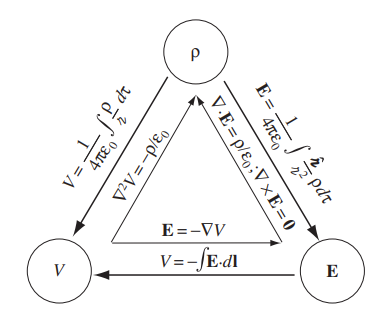
\includegraphics[width=10cm]{Electrodynamics/images/fig2.35.PNG}
\end{center}

Now onto the point of this section: what happens to $\vec{E}$ and $V$ when you cross a \textit{boundary}, i.e. a surface with charge density $\sigma$. 

It is simple to determine this for $\vec{E}$ using Gauss's law: simply draw a really thin wafer of area $A$ and thickness $\epsilon$ containing the surface; then
\[\oiint_{\mathcal{S}}\vec{E}\cdot d\vec{a}=\frac{Q_{\text{enc}}}{\varepsilon_0}=\frac{\sigma A}{\varepsilon_0}.\]
Even if there are other electric charges in the area, the flux through the sides of the pillbox is 0 as we take $\epsilon\to 0$. Hence, the difference in the normal component of the electric field below and the \textit{normal} component (obtained after dotting with $d\vec{a}$) of the electric field above is $\frac{\sigma}{\varepsilon_0}$. Note that this is true for a single infinitely flat plane with surface charge density $\sigma$ as well: the electric fields are both of magnitude $\frac{\sigma}{2\varepsilon_0}$, but pointing in opposite directions.

However, the \textit{tangential} component of $\vec{E}$ is \textit{always} continuous. After all, the loop integral of $\vec{E}$ is always $0$, so if we considered a small loop that is the along the side of the pillbox (so length $\ell$ parallel to the surface and length $\epsilon$ through the surface), then we see that the tangential components must be equal (since their difference is 0).

Hence, we can summarize:
\[\boxed{\vec{E}_{\text{above}}-\vec{E}_{\text{below}}=\frac{\sigma}{\varepsilon_0}\hat{n}},\]
where $\hat{n}$ is a unit vector pointing from below to above.

On the other hand, the potential is continuous across \textit{any} boundary, since the difference in $V$ is given by the path integral of $\vec{E}$, but since the path length shrinks to zero, so too does the integral:
\[V_{\text{above}}-V_{\text{below}}=-\int_{\text{below}}^{\text{above}}\vec{E}\cdot d\vec{\ell}=0.\]

The \textit{gradient} of $V$ keeps the discontinuity though, so
\[\nabla V_{\text{above}}-\nabla V_{\text{below}}=-\frac{\sigma}{\varepsilon_0}\hat{n}.\]
More conveniently, we can consider the $\hat{n}$ component of both sides by taking the dot product with $\hat{n}$, recalling that the dot product of the gradient of $V$ with a unit vector gives the rate of change of $V$ along the direction of that unit vector:
\[\frac{\partial V}{\partial n}=(\nabla V)\cdot\hat{n};\]
in this case, we call it the \vocab{normal derivative} of $V$, i.e. the rate of change of $V$ in the direction perpendicular (normal) to the surface. Hence, we can write
\[\boxed{\frac{\partial V_{\text{above}}}{\partial n}-\frac{\partial V_{\text{below}}}{\partial n}=-\frac{\sigma}{\varepsilon_0}}.\]

\section{Work and Energy in Electrostatics}

\subsection{The Work It Takes to Move a Charge}

Suppose we have a \textit{stationary} configuration of source charges, and want to move a test charge $Q$ from $\vec{a}$ to $\vec{b}$. How much work will we have to do?

Well, the force at any point is given by $\vec{F}=Q\vec{E}$; so you need to exert $-Q\vec{E}$. Hence the needed work is
\[W=\int_{\vec{a}}^{\vec{b}}\vec{F}\cdot d\vec{\ell}=-Q\int_{\vec{a}}^{\vec{b}}\vec{E}\cdot d\vec{\ell}=Q[V(\vec{b})-V(\vec{a})].\]
As $\nabla\times \vec{E}=\vec{0}$, this answer is independent of the path from $\vec{a}$ to $\vec{b}$: therefore, we call the electrostatic force \textit{conservative}.

Hence,
\[V(\vec{b})-V(\vec{a})=\frac{W}{Q}.\]
This gives us another view of potential:
\begin{moral}
The potential difference between points $\vec{a}$ and $\vec{b}$ is equal to the work per unit charge required to carry a particle from $\vec{a}$ to $\vec{b}$.
\end{moral}
In particular, if you want to bring $Q$ in from far away at stick it at $\vec{r}$, you must do work $W=Q\cdot V(\vec{r})$ (as we set our reference point at infinity). In this sense, potential is \textit{potential energy per unit charge} of a single particle moving within a field generated by stationary source charges.

\subsection{The Energy of a Point Charge Distribution}

But what we want to assemble an entire \textit{collection} of point charges? How much work would we need?

The first charge $q_1$ takes zero work: there's nothing to help or fight against. Bringing in $q_2$ will cost $q_2V_1(\vec{r_2})$, where $V_1$ is the potential due to $q_1$, which is then evaluated at $\vec{r_2}$:
\[W_2=\frac{1}{4\pi \varepsilon_0}\frac{q_1q_2}{\scr_{12}},\]
where $\scr_{12}$ is the distance from $\vec{r_1}$ to $\vec{r_2}$. Moving in $q_3$ then takes
\[W_3=\frac{1}{4\pi\varepsilon_0}\frac{q_1q_3}{\scr_{13}}+\frac{1}{4\pi\varepsilon_0}\frac{q_2q_3}{\scr_{23}},\]
and so on. Continuing this pattern, the total work necessary is
\[W=\frac{1}{4\pi \varepsilon_0}\sum_{i=1}^n\sum_{j=i+1}^n\frac{q_iq_j}{\scr_{ij}}=\frac{1}{8\pi\varepsilon_0}\sum_{i=1}^n\sum_{j\neq i}^n\frac{q_iq_j}{\scr_{ij}}.\]
This is equal to
\begin{equation}\label{pointchargeenergy}
\frac{1}{2}\sum_{i=1}^nq_i\left(\sum_{j\neq i}^n\frac{1}{4\pi\varepsilon_0}\frac{q_i}{\scr_{ij}}\right)=\frac{1}{2}\sum_{i=1}^nq_iV(\vec{r_i}).
\end{equation}
This is exactly half of what you'd expect if you just added the work of placing any point charge into the configuration (holding everything else and their generated potential fixed).

This value represents the energy stored in the system of charges (avoiding the annoying term \textit{``potential" energy}).

\subsection{The Energy of a Continuous Charge Distribution}\label{energyinfield}

For a volume charge density $\rho$, this becomes
\[W=\frac{1}{2}\iiint_{\mathbb{R}^3}\rho Vd\tau.\]
There is actually a wonderful way to rewrite this equation to get rid of $\rho$ and $V$ in place of $\vec{E}$. First, use Gauss's law to convert $\rho$ to $\vec{E}$:
\[\rho=\varepsilon_0
\nabla\cdot \vec{E}\implies W=\frac{\varepsilon_0}{2}\iiint_{\mathbb{R}^3}(\nabla\cdot \vec{E})Vd\tau.\]
Now, use integration by parts to transfer the derivative from $\vec{E}$ to $V$:
\[W=\frac{\varepsilon_0}{2}\left[-\iiint_{\mathbb{R}^3}E\cdot(\nabla V)d\tau+\oiint_{\partial \mathbb{R}^3}V\vec{E}\cdot d\vec{a}\right].\]
Wait a second... what's $\partial \RR^3$? Well... if we expand the volume containing charge over and over then the surface integral will drop to $0$ since area grows with $r^2$ but $V$ falls off with $1/r$ and $\vec{E}$ falls off with $1/r^2$.

Now we can use $\nabla V=-\vec{E}$ to get
\begin{equation}\label{energyelectric}
\boxed{W=\frac{\varepsilon_0}{2}\iiint_{\RR^3}E^2d\tau}.
\end{equation}
The energy stored in an electric field per unit volume, then, is $\frac{\varepsilon_0E^2}{2}$.

\subsection{Comments on Electrostatic Energy}

\paragraph{A perplexing ``inconsistency".} The equation 
\[W=\iiint\frac{\varepsilon_0 E^2}{2}d\tau\]
seems to imply that the energy of a stationary charge distribution is \textit{always positive}. Yet the energy of two equal but opposite charges a distance $\scr$ apart is apparently negative quantity $-(1/4\pi\varepsilon_0)(q^2/\scr)$, according to Equation \ref{pointchargeenergy}.

What's going on? Well, \textit{both are correct}. The problem here is that the energy in $-(1/4\pi\varepsilon_0)(q^2/\scr)$ \textbf{doesn't take into account the energy necessary to \textit{create} the point charges} (it supposes the point charges are already given, we're just assembling them), while Equation \ref{energyelectric} does. 

This is good, in fact, as the energy of a point charge is actually \textit{infinite}. By Equation \ref{energyelectric},
\begin{align*}
W&=\frac{\varepsilon_0}{2}\iiint_{\mathbb{R}^3}\frac{1}{(4\pi\varepsilon_0)^2}\cdot \frac{q^2}{r^4}d\tau\\
&=\frac{q^2}{32\pi^2\varepsilon_0}\int_{\varphi=0}^{2\pi}\int_{\theta=0}^\pi\int_{r=0}^\infty \frac{1}{r^4}\cdot r^2\sin\theta drd\theta d\varphi.\\
&=\frac{q^2}{8\pi\varepsilon_0}\int_0^\infty \frac{1}{r^2}dr=\infty.
\end{align*}

So Equation \ref{energyelectric} is more \textit{complete} in giving the total energy stored in the charge configuration. Yet for point charges, as we've seen, we definitely shouldn't include this, so Equation \ref{pointchargeenergy} assumes the point charges are already made (e.g. electrons), and cannot be taken apart. So the energy inside them doesn't matter.

\paragraph{Where is the energy stored?} Is the energy stored in the charge, or in the field? Presently, this is an unanswerable question: we can compute \textit{what} the total energy is, and several ways to compute it, but worrying \textit{where} it is is irrelevant. In radiation theory and general relativity, it is useful to regard the energy as stored in the field with energy density $\frac{\varepsilon E^2}{2}$ per unit volume.

However, in electrostatics, we can just as well say that the energy is stored in the charge, with density $\frac{1}{2}\rho V$.

\paragraph{The superposition principle.} Because electrostatic energy is \textit{quadratic} in the fields, it does \textit{not} obey a superposition principle. The energy of a compound system is \textit{not} the sum of the energies of its parts considered equally, as there are cross terms:
\[W_{\text{tot}}=\frac{\varepsilon_0}2\iiint (\vec{E_1}+\vec{E_2})^2d\tau=W_1+W_2+\varepsilon_0\iiint \vec{E_1}\cdot\vec{E_2}d\tau.\]
For example, if you double the charge everywhere, you quadruple the total energy. The third term here is called the \vocab{interaction energy}: the total energy in the union of two charge configurations is the energy in either, plus the energy it takes to put them together (the interaction energy).  

\section{Conductors}

\subsection{Basic Properties}

\begin{definition}
In an \vocab{insulator}, such as glass or rubber, electrons are not free to move around: they are held closely to particular atoms by short leashes. 
\end{definition}

\begin{definition}
In a metallic \vocab{conductor}, con the other hand, one or more electrons per atom are free to roam. (In liquid conductors, ions move).
\end{definition}

From this definition, we can derive several electrostatic properties:

\paragraph{$\vec{E}=\vec{0}$ inside a conductor.} The general idea is that if not, then the free charges inside the conductor would move to generate an \textit{opposing electric field} that cancels out any external one. This movement of charges occurs practically instantaneously.

\paragraph{$\rho=0$ inside a conductor.} Follow from Gauss's Law: $\rho=\varepsilon_0\nabla\cdot \vec{E}$.

\paragraph{Any net charge resides on the surface.} Where else could the net charge be?

\begin{remark}
This particular condition is pretty surprising: charges do push each other so it's natural for them to spread out, but placing them all on the boundary seems like a waste of the space inside (shouldn't you at least sprinkle a little charge in the middle?). Nonetheless, it is true that minimizing the energy stored in the system is best done by moving all the charge to the surface.
\end{remark}

\paragraph{A conductor is an equipotential.} Since the path integral of $\vec{E}$ is $0$, as $\vec{E}$ itself is always $\vec{0}$.

\paragraph{$\vec{E}$ is perpendicular to the surface, just outside a conductor.} Otherwise charge on the conductor would immediately move around to cancel out any tangential component of the electric field. Charge cannot move in the normal direction, of course, since it is confined to the conductor.

\subsection{Induced Charges}

Placing a $+q$ charge near an uncharged (!) conductor will cause them to attract. This is because the $+q$ charge will pull negative charges closer to it and repel positive charges farther away. Since the negative charge in the conductor is closer to the $+q$ charge, we will see a net attractive force.

While the field inside the actual material making up a conductor must be zero, there can be an electric field within any hollow cavities closed off within a conductor. 

However, it turns out that charges within a cavity in a conductor are \textit{electrically isolated from the outside world}: no fields penetrate the conductor, but you can still detect the presence of a charge inside due to charge present on the outer surface of the conductor.

Let's investigate closely what happens: if we have a point charge $+q$ inside a hollow cavity in a conductor, then negative charges will rush to the boundary of the hollow cavity (the inside surface of the conductor), while positive charges will be pushed outward to the outside surface of the conductor. 

\begin{center}
    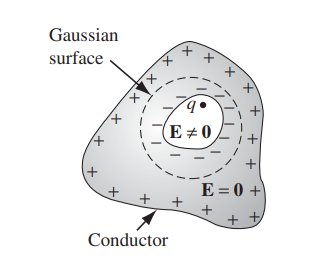
\includegraphics[width=6cm]{Electrodynamics/images/fig2.45.PNG}
\end{center}

If we take a Gaussian surface running entirely through the conductor that encloses the hollow cavity, we know the flux through this surface must be zero (as the electric field along the entire surface is zero). Therefore, the charge enclosed by this Gaussian surface is zero; hence, the inside surface of the conductor surrounding the hollow cavity develops a charge $-q$. Since the conductor started neutral, its outside surface must develop a charge $+q$. 

\begin{example}
An uncharged spherical conductor centered at the origin has a cavity of some weird shape carved out of it in the inside. Somewhere within the cavity is a charge $q$. What is the field outside the sphere?
\end{example}

\begin{proof}
    It turns out the answer depends neither on the shape of the cavity nor the location of the charge! Wild, isn't it. 
    
    Indeed, it turns out that any imbalance from the position of $q$ or the shape of the cavity is balanced out by the negative charge developed on the inner surface, and the charge $q$ spread on the outside of the sphere is uniform! Hence, the answer is
    \[\boxed{\vec{E}=\frac{1}{4\pi\varepsilon_0}\frac{q}{r^2}\hat{r}}.\]
\end{proof}

\begin{remark}
The argument here isn't conclusive. There are \textit{three} fields at work here: $\vec{E}_q$ from the point charge, $\vec{E}_{\text{induced}}$ from the charge of $-q$ on the inside surface of the conductor, and $\vec{E}_{\text{leftover}}$ from the charge of $q$ on the outside surface of the conductor.

We cannot supply a fully rigorous argument yet, but for now, take note that there \textit{exists} a way of distributing the $-q$ on the inner surface so that $\vec{E}_q$ and $\vec{E}_{\text{induced}}$ cancel at any exterior points. Indeed, the same cavity (with the point charge inside) could've been carved out of an insanely large conductor, and the positive charges out the outside just would be too far away to affect the inside, so the first two fields would have to do all the work of cancellation by themselves.

Yet how do we know that this is actually what happens? Well, it turns out that due to some uniqueness theorems of Chapter 3, electrostatics has the property that there is precisely one way of distributing the charge on a conductor so that the field inside is zero. Having found a single \textit{possible} way, we are guaranteed that no alternative exists.
\end{remark}

If there is no charge inside the cavity, then we can argue that $\vec{E}=0$; indeed, if there was some field line beginning and ending on the cavity wall, integrating across it would violate the fact that all points on the conductor have equal potential. This is the principle behind grounded \vocab{Faraday cages}, which will shield out stray electric fields. In practice, the conductor doesn't even have to be solid; something like chicken wire often suffices.

\subsection{Surface Charge and the Force on a Conductor}\label{surfcharforcond}

Since the field inside a conductor is zero, and all the charge is concentrated on the surface of the conductor, the boundary conditions from Section \ref{boundcond} require that the field immediately outside the conductor is
\[\vec{E}=\frac{\sigma}{\varepsilon_0}\hat{n},\]
where $\hat{n}$ is the unit vector normal to the surface of the conductor. In terms of potential, we get
\[\frac{\partial V}{\partial n}=-\frac{\sigma}{\varepsilon_0}\]
for the value of the directional derivative of $V$ in the direction of the normal $\hat{n}$. Hence, if you can determine $\vec{E}$ or $V$, you can calculate the surface charge on a conductor.

In the presence of an electric field, a surface charge will experience a force per unit area of $\vec{f}=\sigma\vec{E}$. But the electric field is \textit{discontinuous} at a surface charge, so what do we use for $\vec{E}$? The answer is the average of the electric field below and above:
\[\vec{f}=\sigma\vec{E}_{\text{average}}=\frac{1}{2}\sigma(\vec{E}_{\text{above}}+\vec{E}_{\text{below}}).\]
All this average does is remove any contribution of the surface itself to the electric field (as obviously the patch cannot exert a force on itself).

This argument applies to \textit{any} surface charge; in the particular case of a conductor, the field inside is zero and outside is $\frac{\sigma}{\varepsilon_0}\hat{n}$; hence the force per area is
\[\vec{f}=\frac{\sigma^2}{2\varepsilon_0}\hat{n}.\]
This amounts to an outwards \vocab{electrostatic pressure} on the surface, drawing the conductor into the field, regardless of the sign of $\sigma$. We can also write the pressure as
\[P=\frac{\varepsilon_0 E^2}{2}.\]

\subsection{Capacitors}

Suppose we have two conductors, one with charge $+Q$ on in it and one with charge $-Q$ on it. Since $V$ is constant over conductors, the potential difference between these two conductors is unambiguous:
\[V=V_+-V_-=-\int_{(-)}^{(+)}\vec{E}\cdot d\vec{\ell}.\]
We don't know how the charges get distributed, or what the exact field looks like, but we do know that $\vec{E}$ and $V$ should both be proportional to $Q$. After all, $\vec{E}$ is given by Coulomb's law
\[\vec{E}=\frac{1}{4\pi\varepsilon_0}\iiint_{\mathbb{R}^3}\frac{\rho}{\scr^2}\hat{\scr}d\tau,\]
so if you double $\rho$ everywhere, you double $\vec{E}$ as well. 

\begin{remark}
There is a slight caveat here: how do we know that, say, doubling $Q$ actually doubles $\rho$ everywhere. Maybe the charge would actually move around, so that in some places $\rho$ is quadrupled while in others maybe it is halved, so that the total charge $Q$ is still doubled. Well, it turns out that doubling $Q$ does in fact double $\rho$ everywhere, but the proof of this will have to wait for Chapter 3.
\end{remark}

Since $\vec{E}$ is proportional to $Q$, and $\vec{E}=-\nabla V$, $V$ is also proportional to $Q$. 

\begin{definition}
The constant of proportionality between $Q$ and $V$ is called the \vocab{capacitance} of the arrangement:
\[C:=\frac{Q}{V}.\]
\end{definition}

Capacitance is a purely geometrical quantity, determined entirely by the sizes, shapes, and separation between the two conductors. Capacitance is measured in \vocab{farads}, which is a coulomb-per-volt. This is generally inconveniently large: microfarads and picofarads are more convenient.

Note that since $Q$ and $V$ are both \textit{defined} to be positive, $C$ is always positive. 

\begin{remark}
Sometimes, you will hear people speak of the capacitance of a \textit{single} conductor. In this case, the ``second conductor" is an imaginary spherical shell of infinite radius surrounding the conductor. It contributes nothing to the field, so the capacitance is just given by $Q/V$ where $V$ is the potential with $\infty$ as the reference point.
\end{remark}

\begin{example}[Capacitance of parallel-plate capacitor]
Find the capacitance of two metal surfaces of area $A$ held a distance of $d\ll A$ apart.
\end{example}

\begin{proof}[Solution]
When $d\ll A$, the field between the two plates can be approximated as $Q/A\varepsilon_0$ from the positive plate to the negative plate. Therefore, the potential difference is
\[V=-\int_{(-)}^{(+)}\vec{E}\cdot d\vec{\ell}=\frac{Qd}{A\varepsilon_0}.\]
Hence,
\[C=\frac{Q}{V}=\boxed{\frac{\varepsilon_0A}{d}}.\]
\end{proof}

\begin{example}
Find the capacitance of two concentric spherical metal shells, with radii $a$ and $b$.
\end{example}

\begin{proof}[Solution]
Place a charge $+Q$ on the inner sphere of radius $a$, and $-Q$ on the outer sphere of radius $b$. Then the field between the two spheres is
\[\vec{E}=\frac{1}{4\pi\varepsilon_0}\frac{Q}{r^2}\hat{r}.\]
Therefore, the potential difference is
\[V=\int_{(+)}^{(-)}\vec{E}\cdot d\vec{\ell}=\frac{Q}{4\pi\varepsilon_0}\int_a^b\frac{1}{r^2}dr=\frac{Q}{4\pi\varepsilon_0}\left(\frac{1}{a}-\frac{1}{b}\right).\]
Hence,
\[C=\frac{Q}{V}=\boxed{4\pi\varepsilon_0\cdot\frac{ab}{b-a}}.\]
\end{proof}

In order to charge up a capacitor, you must remove electrons from the positive plate and carry them to the negative plate. Doing so fights against the electric field. How much work does it take to charge up the capacitor to a final amount $Q$?

\begin{proposition}\label{workchargecapacitor}
The amount of work necessary to charge a capacitor up to a final amount $Q$ is given by
\[W=\frac{Q^2}{2C}=\frac{1}{2}CV^2.\]
\end{proposition}

\begin{proof}
Indeed, if we've already charged the capacitor up by $q$, then the potential difference is $q/C$. Hence, the work required to move it is
\[dW=\frac{q}{C}dq.\]
The total work, then, is
\[W=\int_{0}^Q\frac{q}{C}dq=\frac{1}{2}\frac{Q^2}{C}.\]
Since $Q=CV$, we often write this as
\[W=\frac{1}{2}CV^2.\]
\end{proof}
